\documentclass[12pt]{article}

\usepackage[utf8]{inputenc}
\usepackage[brazil]{babel}
\usepackage[a4paper,left=3cm, right=2cm,top=2.5cm, bottom=2.5cm]{geometry}
\usepackage{amsmath}
\usepackage{graphicx}
\usepackage{float}
\usepackage{multirow}
\usepackage{authblk}
\usepackage{fancyhdr}
\usepackage[table,xcdraw]{xcolor}

\title{\textbf{Econometria de séries financeiras: da modelagem clássica às ondaletas}}
\author{\textbf{Aluno: Matheus Carneiro Nogueira}}
\affil{}
\author{\textbf{Orientador: Edgard Pimentel}}
\affil{}
\pagestyle{fancy}
\fancyhf{}
\lhead{{\small{\textit{Departamento de Matemática}}}}
\renewcommand{\headrulewidth}{0pt}
\date{}
\renewcommand{\footrulewidth}{0pt}
\fancyfoot[C]{\thepage}
\date{}

\begin{document}
	\maketitle
	
	
	\section{Introdução}
	Séries Temporais são objetos de extrema relevância nas mais diversas áreas de conhecimento. Informações como evolução de gastos energéticos, retornos de ativos financeiros e evolução populacional de um território são apenas algumas das aplicações destes objetos. Sendo assim, o estudo de modelos de econometria que fornecem descrições precisas de séries temporais é extremamente relevante. Com isso em mente, focando em análise de modelos econométricos para séries financeiras, foi desenvolvida esta pesquisa comparativa de 3 diferentes modelos. Primeiramente, foi estudado e implementado o modelo ARIMA para a previsão de séries temporais dos retornos de ações de 10 companhias aéreas. Os resultados desta primeira etapa já foram apresentados no relatório anual de 2020 e podem ser acessados em \cite{git}. Em seguida, foram estudados os modelos VAR e  um modelo híbrido que combina a teoria das Ondaletas \textrm{(Wavelets)} com a modelagem ARIMA já apresentada utilizando as mesmas 10 séries temporais.  
	
	\section{Objetivos}
	Após estudado o modelo ARIMA, uma ferramenta clássica para a análise de séries temporais, e constatado que ele se mostra pouco confiável para a previsão de retornos financeiros, o objetivo passou a ser estudar e entender dois novos modelos com o intuito de implementá-los e comparar a qualidade de suas previsões. Para isso, foram utilizadas as mesmas 10 séries temporais de preços de ações de companhias aéreas. Primeiramente, o objetivo é produzir um modelo VAR com o intuito de buscar, por meio do ferramental disponível por este modelo, interconexões das séries utilizadas de tal modo a melhorar a qualidade da previsão. Por fim, o objetivo passa a ser estudar a teoria de \textrm{Wavelets} a fim de criar um modelo híbrido que une esta teoria ao modelo ARIMA, já conhecido, de modo a utilizar a análise simultânea dos domínios do tempo e frequência como ferramenta para aumentar a qualidade de previsão.
	
	\section{Metodologia}
	Para fins didáticos, a metodologia utilizada no decorrer da pesquisa será dividida em duas grandes partes. Primeiramente serão apresentados os fundamentos teóricos do modelo VAR com a discussão de seus resultados. Em seguida, os fundamentos teóricos da teoria de \textrm{Wavelets} com a implementação do modelo híbrido e, também, a discussão de seus resultados. 
	
	\subsection{Modelo VAR}
	
	Antes de analisar o modelo VAR \textrm{(Vector Autoregressive Model)}, vale relembrar o modelo AR \textrm{(Autoregressive Model)} apresentado em \cite{Tsay}. A equação que define este modelo é
	\begin{equation}\label{eq:AR}
		r_t=\phi_0+\phi_1r_{t-1}+...+\phi_pr_{t-p}+a_t
	\end{equation}
	onde os valores $\phi_i$ são os coeficientes a serem estimados, $r_t$ é o valor presente da série, $r_{t-i}$ são os valores defasados e ${a_t}$ é um ruído branco de média zero e variância $\sigma^2_a$. 
	
	Este modelo foi utilizado para compor o modelo ARIMA e prever o comportamento de 10 séries temporais estacionárias e univariáveis de forma independente, cujos resultados já foram apresentados e estão disponíveis em \cite{git}.
	
	O modelo VAR, como o nome sugere, também é um modelo auto regressivo mas, ao invés de aceitar apenas séries univariáveis, isto é, valores escalares para as variáveis $r_t$, $r_{t-i}$ e para os coeficientes $\phi_i$, é capaz de modelar séries multivariáveis. Sendo assim, podemos apresentar a equação que define o modelo VAR definida em \cite{VAR}. Seja $Y_t=(y_{1t},y_{2t},...y_{nt})^T$ um vetor de dimensão $(n\times 1)$ com os valores atuais de $n$ séries temporais. Sendo assim, o modelo VAR com um \textrm{lag-p} de valores defasados é
	\begin{equation}\label{eq:VAR}
		Y_t=c+\Pi_1Y_{t-1}+\Pi_2Y_{t-2}+...+\Pi_pY_{t-p}+\epsilon_t\mbox{  , onde }t=1,...T
	\end{equation}

	Note que esta equação é praticamente idêntica à equação \ref{eq:AR}, uma vez que ambas definem modelos auto regressivos. A diferença está no fato de $\Pi_i$ não serem mais coeficientes escalares, mas sim matrizes de coeficientes de dimensão $(n\times n)$ e $e_t$ ser um vetor $(n\times1)$ de ruídos brancos. 
	
	Embora este modelo possa ser usado para séries multivariáveis, é mais adequado, dentro de nosso escopo de modelagem de 10 séries temporais, enxergá-lo como o encapsulamento de $n$ séries temporais univariáveis utilizando notação matricial. O que pode facilitar esta maneira distinta de enxergá-lo é o exemplo de reescrita da equação \ref{eq:VAR} do modelo para um exemplo de um VAR(2) de duas variáveis.
	\begin{equation*}
		\begin{pmatrix}
			y_{1t} \\
			y_{2t}
		\end{pmatrix}=
		\begin{pmatrix}
			c_{1} \\
			c_{2}
		\end{pmatrix}+
		\begin{pmatrix}
			\pi_{11}^{1} & \pi_{12}^{1}\\
			\pi_{21}^{1} & \pi_{22}^{1}
		\end{pmatrix}
		\begin{pmatrix}
			y_{1t-2} \\
			y_{2t-2}
		\end{pmatrix}+
		\begin{pmatrix}
		\pi_{11}^{2} & \pi_{12}^2\\
		\pi_{21}^{2} & \pi_{22}^2
		\end{pmatrix}
		\begin{pmatrix}
			y_{1t-2} \\
			y_{2t-2}
		\end{pmatrix}+
		\begin{pmatrix}
			\epsilon_{1t} \\
			\epsilon_{2t}
		\end{pmatrix}	
	\end{equation*}

	Note que podemos ler cada linha das matrizes e vetores da equação cima como modelos AR(2) definidos de acordo com a equação \ref{eq:AR}.
	
	Uma vez apresentado o modelo VAR(p) e a sua relação com o modelo AR(p) é natural que surja a seguinte pergunta: qual a vantagem de utilizarmos um modelo vetorial para a análise de 10 séries temporais se podemos realizá-las individualmente? 
	
	O modelo vetorial, dentro do escopo desta pesquisa, apresenta duas vantagens interessantes para a modelagem de nossas 10 séries temporais.
	\begin{enumerate}
		\item Ao encapsular as séries dentro de um vetor, o modelo enxerga um só bloco de informação e busca correlações e interdenpendências entre as séries. Caso essas relações existam, o modelo pode fornecer previsões mais precisas.
		\item O modelo vetorial fornece ferramentas estatísticas para analisar a interconexão das séries temporais utilizada. 
	\end{enumerate}

	A primeira vantagem é obviamente interessante, uma vez que o grande objetivo é, justamente, obter modelos de previsão de séries temporais mais precisos. A segunda, por sua vez, também é importante uma vez que as 10 séries utilizadas, por serem de um mesmo nicho - todas são séries dos preços/retornos de ações de companhias aéreas - podem revelar análises de interconexão interessantes. A apresentação dessa ferramentas está descrita na seção \ref{sec:interconex}.
	
	Uma vez compreendida a equação que define o modelo VAR e as suas características possivelmente vantajosas, podemos definir a metodologia utilizada para a estimativa de seus parâmetros, para a definição do \textrm{lag-p} e o seu método de previsão.
	
	Com o intuito de estimar os parâmetros necessários para o modelo, utiliza-se o fato dele poder ser enxergado como o encapsulamento de $n$ séries a serem modeladas via AR(p). Desse modo, é possível estimar os parâmetros da cada uma das equações separadamente sem perda de generalidade \cite{VAR}. Sendo assim, é utilizado o método de mínimos quadrados para realizar esta estimativa de coeficientes.
	
	Novamente, sabendo que o modelo VAR é um modelo auto regressivo assim como o AR, o \textrm{lag-p}, isto é, o número de valores passados das séries que serão utilizados para estimar o modelo e, consequentemente, prever os valores futuros, é estimado a partir da minimização de alguns critérios. Os critérios mais comuns a serem minimizados são \textrm{Akaike} (AIC), \textrm{Schwarz-Bayesian} (BIC) e \textrm{Hannan-Quinn} (HQ) \cite{VAR}. Esses critérios encontram-se definidos abaixo.
	\begin{align*}
		\textrm{AIC(p)}=&\ln\left|\sum(p)\right|+\dfrac{2}{T}pn^2\\
		\textrm{BIC(p)}=&\ln\left|\sum(p)\right|+\dfrac{\ln T}{T}pn^2\\
		\textrm{HQ(p)}=&\ln\left|\sum(p)\right|+\dfrac{2\ln \ln T}{T}pn^2
	\end{align*}

	Cada um desses critérios possui características próprias. O AIC assintoticamente superestima a ordem do \textrm{lag-p} com probabilidade positiva, enquanto os critérios BIC e HQ tende a estimar de forma consistente a ordem do \textrm{lag-p} se a ordem verdadeira \textrm{p} for menor ou igual a uma ordem \textrm{p-max} pré estabelecida. Após a estimativa dos coeficientes, a fim de verificar a qualidade do modelo obtido analisa-se os resíduos (erros) tanto das séries quanto das ACF e PACF, que são funções de autocorrelação cuja apresentação foi feita anteriormente \cite{Tsay-Tiao1984}.
	
	A etapa mais importante desta pesquisa é a \textbf{previsão}. Uma vez assumido que os coeficientes são conhecidos e que não existe nenhum termo exógeno à série, o método de previsão linear utilizado para a previsão de um passo a frente é:
	\begin{equation}\label{eq:VAR_FOR_1}
		Y_{T+1|T}=c+\Pi_1Y_{T}+...+\Pi_pY_{T-p+1}
	\end{equation} 
	
	Esse método baseia-se em todos os valores passados da série até o tempo $T-P+1$, sendo $T$ o índice do último valor conhecido da série. Sendo assim, imagine que nossa série possui entradas mensais e que o último valor conhecido é de Dezembro de 2020. Se nosso \textrm{lag-p}  foi definido como 2, podemos rescrever a equação \ref{eq:VAR_FOR_1} de forma mais didática.
	\begin{equation*}
		Y_{Jan2021|Dez2020}=c+\Pi_1Y_{Dez2020}+\Pi_2Y_{Nov2020}
	\end{equation*}

	O que essa equação nos diz é: o valor da série em Janeiro de 2021 (a ser previsto), conhecendo todos os valores até Dezembro de 2020, é função dos valores de Novembro de 2020 e Dezembro de 2020, uma vez que nosso \textrm{lag-p} é igual a 2.
	
	A previsão de h-passos a frente pode ser obtida utilizando a regra da cadeia de previsão \cite{VAR} como se segue:
	\begin{equation}\label{eq:VAR_FOR_h}
		Y_{T+h|T}=c+\Pi_1Y_{T+h-1|T}+...+\Pi_pY_{T+h-p|T}
	\end{equation}
	
	onde, para $j\leq0$, isto é, para valores conhecidos $(t\leq T)$, $Y_{T+j|T}=Y_{T+j}$.
	
	Se os coeficientes não são conhecidos, mas são frutos de estimativas tais quais as apresentadas anteriormente, a melhor maneira de prever o comportamento de $Y_{T+h}$ é
	\begin{equation}
		\hat{Y}_{T+h|T}=c+\hat{\Pi}_1\hat{Y}_{T+h-1|T}+...+\hat{\Pi}_p\hat{Y}_{T+h-p|T}
	\end{equation}

	onde $\hat{\Pi}_i$ são as matrizes de coeficientes estimados. A diferença é apenas de notação, de certo modo. A existência do símbolo circunflexo denota o fato daquele parâmetro ter sido estimado e não conhecido a priori. O tamanho do horizonte de previsão, isto é, a quantidade de passos futuros a serem previstos, deve ser definido com cautela,  visto que o erro das previsões tende a aumentar com o aumento do horizonte. Veremos que, para horizontes grandes, o valor da previsão parece convergir para um valor constante.
	
	Por fim, com o intuito de verificar a qualidade da previsão, foi utilizado o RMSE, \textrm{Root Mean Square Error}, entre os valores originais das séries separados como grupo de teste e os valores previstos para esse intervalo separado. O RMSE é calculado como se segue:
	\begin{equation}\label{eq:RMSE}
		\textrm{RMSE} = \sqrt{\dfrac{\sum_{t=1}^{h}(\hat{Y}_t-Y_t)^2}{h}}
	\end{equation} 
	
	onde $h$ é tanto o número de passos a frente e a quantidade de valores comparados.
	
	\subsubsection{Análise de Interconexões} \label{sec:interconex}
	
	Após a rápida explicação teórica por detrás do modelo VAR, haja vista a sua enorme similaridade com o modelo AR já estudado com base em \cite{Tsay} e apresentado no relatório disponível em \cite{git}, podemos analisar o fundamento teórico de três ferramentas estatísticas disponíveis pelo modelo vetorial que permitem a análise e procura de possíveis interconexões ou interdependência entre as séries modeladas. São elas: \textrm{Granger Causality}, \textrm{Impulse Response Function} e \textrm{Forecast Error Variance Decomposition} (FEVD).\\
	
	A \textbf{Causalidade de Granger} consiste em uma métrica que busca descobrir se uma das séries modelada pelo VAR é causa das demais séries modeladas. Em outras palavras, esta ferramenta busca responder à pergunta: será que os valores de cada uma das séries do modelo são consequência dos valores de alguma das outras séries? É importante ressaltar que essa análise se limita a estudar a causalidade em termos de previsão.
	
	Para entender melhor essa análise, tome o exemplo de duas séries temporais arbitrárias: a série que mede a quantidade de chuva semanal no estado do Rio de Janeiro e a série que mede o nível de água semanal do rio Paraíba do Sul. É natural pensarmos que, se em uma dada semana a quantidade de chuva aumenta em relação a semana anterior, o nível de água do rio também aumentará. Essas duas séries, mais do que correlacionadas, estão causalmente relacionadas, ou seja, a evolução ou os valores de uma das séries (quantidade de chuvas) é influencia de maneira causal a evolução ou os valores da outra (nível de água no rio Paraíba do Sul). Se essas séries forem modeladas via VAR e submetidas ao teste de causalidade de Granger, espera-se que ele chegue neste mesmo resultado obtido pelo senso comum.
	
	A maneira de determinar se uma série \textrm{granger-cause} outra é analisar os coeficientes das matrizes $\Pi_i$ da equação \ref{eq:VAR}. Com o intuito de visualizar essa análise, é apresentado o exemplo para um modelo VAR de 2 variáveis. A série $y_2$ \textbf{falha} em causar a série $y_1$, se todos os coeficientes $\pi_{12}^i$ forem zero, ou seja, se as matrizes $\Pi_i$ forem triangulares inferiores, como se segue para o caso de um VAR(2).
	\begin{equation*}
		\begin{pmatrix}
			y_{1t} \\
			y_{2t}
		\end{pmatrix}=
		\begin{pmatrix}
			c_{1} \\
			c_{2}
		\end{pmatrix}+
		\begin{pmatrix}
			\pi_{11}^{1} & 0\\
			\pi_{21}^{1} & \pi_{22}^{1}
		\end{pmatrix}
		\begin{pmatrix}
			y_{1t-2} \\
			y_{2t-2}
		\end{pmatrix}+
		\begin{pmatrix}
			\pi_{11}^{2} & 0\\
			\pi_{21}^{2} & \pi_{22}^2
		\end{pmatrix}
		\begin{pmatrix}
			y_{1t-2} \\
			y_{2t-2}
		\end{pmatrix}+
		\begin{pmatrix}
			\epsilon_{1t} \\
			\epsilon_{2t}
		\end{pmatrix}
	\end{equation*}\\
	
	A \textbf{função de resposta impulsional}, por sua vez, é uma análise que busca responder a seguinte pergunta: como as séries do modelo vão reagir a um choque, a uma mudança abrupta ou a um impulso gerado em uma das séries? Essa análise é interessante por trazer uma ferramenta capaz de prever o comportamento e a reação de séries temporais em relação às outras. Imagine, por exemplo, um cenário de plantação agrícula em um ambiente de pouca chuva anual cujas séries relevantes são a produção semanal de trigo e a quantidade semanal de chuva. Novamente, é de bom senso imaginar que uma semana de tempestades atípicas, que serão percebidas como um choque abrupto na série de quantidade de chuva, vai alterar o comportamento da série que mede a quantidade de trigo colhido na semana seguinte, por exemplo. Sendo assim, conhecer a resposta impulsional da série de quantidade semanal de trigo em função da série de quantidade semanal de chuva pode ser uma informação útil para prevenção de desestres.
	
	A equação que melhor define a função de resposta impulsional é
	\begin{equation*}
		\dfrac{\partial y_{i,t+s}}{\delta \eta_{j,t}}=\dfrac{\partial y_{i,t}}{\delta \eta_{j,t-s}}=\theta^s_{i,j}
	\end{equation*}

	onde $i,j=1,...,n$ e $s>0$. O gráfico de $\theta^s_{i,j}\times s$ é, justamente, a função de resposta impulsional. Embora o entendimento teórico não seja trivial, a interpretação visual dos resultados apresentada na seção \ref{sec:resultados_VAR_itnerconec} é simples. \\
	
	A última das ferramentas de análise de interconexão estudadas é a \textbf{Decomposição de Variância de Erro de Previsão}, ou \textbf{FEVD}, em inglês. Essa análise, assim como apresentada em \cite{VAR}, responde à seguinte pergunta: quanto da variância do erro de previsão de $y_{i,T+h}$ foi causado por causa do choque estrutural $\eta_j$. O resultado desta análise é uma matriz de $n$ colunas, uma para cada série modelada via VAR, e $n^2$ linhas, que são, justamente, os valores calculados pela decomposição. Quanto mais próximos de zero os valores de uma determinada coluna, menos os choques da série desta coluna interferiram na variância do erro da previsão da série analisada. Sendo assim, é de se esperar que, ao analisar uma série $Y$, por exemplo, na coluna da matriz referente a própria série $Y$, todos os valores sejam próximos do valor máximo, 1.
	
	A equação que define a FEVD é
	\begin{equation*}
		\textrm{FEVD}_{i,j}(h)=\dfrac{\sigma^2_{\eta_j}\sum_{s=0}^{h-1}(\theta^s_{ij})^2}{\sigma^2_{\eta_1}\sum_{s=0}^{h-1}(\theta^s_{i1})^2+...+\sigma^2_{\eta_n}\sum_{s=0}^{h-1}(\theta^s_{in})^2}\mbox{   , }i,j=1,...,n
	\end{equation*}
	
	Com isso, encerramos a análise teórica metodológica necessária para entender os resultados obtidos com o modelo VAR ao modelar 10 séries temporais de retornos de ações de companhias aéreas.
	
	\subsection{Resultados VAR}
	\subsubsection{Resultados Previsão}\label{sec:resultados_VAR_previsao}
	
	Assim como para a implementação dos modelos ARIMA já apresentados no relatório passado e dos modelos híbridos \textrm{Wavelets} com ARIMA, foi usada a linguagem R por ser uma linguagem popular e adequada para estudos econométricos. Os pacotes utilizados para ambos os modelos são \textrm{ggplot2} para a criação de gráficos, \textrm{Metrics} para o cálculo do RMSE, \textrm{tseries} para tratamento de séries temporais e \textrm{vars} para a implementação do modelo VAR desde sua estimativa até previsão. Todos os pacotes estão disponíveis em \cite{CRANR}.
	
	Com o intuito de fornecer uma comparação justa, foram usadas para o modelo VAR as mesmas 10 séries de companhias aéreas já utilizadas para os modelos ARIMA. As companhias selecionadas são: IAG, Japan Airlines, China Southern, China Eastern, Latam, Delta, United, American, Lufthansa e AirFrance-KLM. Os dados coletados vão de 2010 a 2019. Essas companhias foram escolhidas por serem 10 das maiores do mundo e representarem diferentes regiões do globo, a fim de obter uma análise mais geral ao invés de uma focada em algum país ou continente.
	
	Para não estender desnecessariamente este relatório, serão apresentadas as imagens de apenas 2 das 10 companhias. Todo o material produzido para esta pesquisa, desde o código em R até as imagens geradas, estão disponíveis em um repositório público \cite{git}. Ao final desta seção estarão as tabelas com os erros comparados das 10 companhias aéreas em relação aos modelos ARIMA.
	
	A metodologia apresentada na seção anterior foi fielmente seguida ao implementar o código em R. Por ser um processo muito similar àquele realizado para os modelos ARIMA, aqui será feita uma breve recapitulação apenas. Para explicações mais detalhadas daquilo que não for abordado com profundidade nesta seção, ver o relatório do ano anterior disponível em \cite{git}.
	
	O primeiro passo após a importação dos dados presentes em arquivos \textrm{csv} é selecionar apenas os valores de interesse, que são os preços fechados ajustados das ações das companhias aéreas. Com esses valores em mãos, podemos inseri-los em vetores numéricos para procurar e substituir valores faltantes, que são comuns em bases de dados utilizadas para obter as séries. Feita essa procura, as séries podem ser visualizadas.
	
	\begin{figure}[H]
		\centering
		\includegraphics[width=1.0\linewidth]{Imagens/AdjCloseVAR}
		\caption{Adjusted Closed Price para Latam e Japan Airlines}
		\label{fig:adjclosevar}
	\end{figure}
	 
	 Neste momento poderia ser feito um teste de estacionariedade, como o \textrm{Augmented Dickey-Fuller Teste}, assim como foi feito para os modelos ARIMA e será feito para os modelos híbridos. No entanto, optou-se por não fazê-lo e obter de uma vez os retornos-log desses preços, haja vista que esta é a variável de interesse da pesquisa. Para tal, basta calcular a diferença dos logs das entradas das séries. Um cuidado importante a ser tomado é, após obter o retorno, submeter as séries a um novo tratamento de busca por valores faltantes ou inválidos, uma vez que as operações realizadas para obter os retornos podem inserir tais valores nas séries. Para isso, utiliza-se a função \textrm{tsclean} do pacote \textrm{tseries}. As imagens abaixo exibem os retornos-log para as mesmas duas séries já apresentadas.
	 
	 \begin{figure}[H]
	 	\centering
	 	\includegraphics[width=1.0\linewidth]{Imagens/LogRetVAR}
	 	\caption{Log-return para Latam e Japan Airlines}
	 	\label{fig:logretvar}
	 \end{figure}
	 
	 
	 Uma etapa que não existia para os modelos ARIMA mas que deve ser realizada para o modelo VAR é reduzir a quantidade de entradas das séries de modo a garantir que todas possuam o mesmo tamanho, igual ao tamanho da menor série utilizada. Essa alteração, embora signifique a perda de informações de algumas séries, é necessária pois o modelo VAR supõe que todas as séries serão encapsuladas em um vetor e, para isso ser possível, todas devem possuir o mesmo número de entradas. Sendo assim, ao invés de criar novos valores para séries menores, opta-se por reduzir, ou seja, deletar entradas, de séries maiores. 
	 
	 Feita esta redução, as séries podem ser divididas em grupos de treino e teste. O grupo de treino é aquele que será usado para estimar os coeficientes do modelo VAR e, com os coeficientes estimados, realizar a previsão. O grupo de teste, por sua vez, sempre é guardado para comparar as previsões realizadas com os valores originais jamais vistos pelo modelo. Dito isso, foram realizadas duas separações. Primeiro foram separados 90\% das séries para treino e 10\% para teste, em prol de avaliar a previsão para grandes horizontes de tempo, visto que 10\% das séries corresponde a 178 entradas. Em seguida, os grupos de teste foram formados com apenas os 20 últimos valores das séries, com o intuito de avaliar a previsão para horizontes mais curtos.
	 
	 Para estimar os valores do \textrm{lag}, via ACF e PACF, diferentemente do que foi feito anteriormente, optou-se por utilizar a função \textrm{VARselect} do pacote \textrm{vars} \cite{CRANR} para definir o valor do \textrm{lag} automaticamente, ao invés da análise individual e visual utilizada para os modelos ARIMA. A única necessidade foi definir um \textrm{lag} máximo de 15, escolhido por ser um valor pouco maior que o maior \textrm{lag} definido para os modelos ARIMA implementados anteriormente. Com o valor do \textrm{lag} definido como 9, foi utilizada a função \textrm{VAR} para estimar o modelo. O único parâmetro necessário é um booleano para sazonalidade que foi definido como falso. O motivo para ele ser falso é o fato de nenhuma das séries utilizadas apresentar perfil sazonal, assim como foi mostrado anteriormente. Novamente, caso seja do interesse do leitor acessar esses resultados passados, todo o material da pesquisa encontra-se em \cite{git}.
	 
	 As imagens abaixo exibem as estimativas para as duas mesmas companhias.
	 
	 \begin{figure}[H]
	 	\centering
	 	\includegraphics[width=1.0\linewidth]{Imagens/VAR_EST}
	 	\caption{Estimativa e resíduos para o modelo VAR}
	 	\label{fig:varest}
	 \end{figure}
	 
	 Como pode ser percebido, os resíduos, assim como desejado, parecem ser independentes, visto que as funções de autocorrelação e autocorrelação parcial estão praticamente zeradas, o que torna os resíduos próximos de um ruído branco.
	 
	 Com isso, estamos aptos a, enfim, prever valores futuros das séries via função \textrm{predict} do mesmo pacote. Os resultados dessas previsões podem ser observados nas figuras abaixo, que exibem, além do valor previsto, o valor original das séries separados como grupo de teste. Como comentado, foram realizadas estimativas e previsões para duas divisões distintas.
	 
	 \begin{figure}[H]
	 	\centering
	 	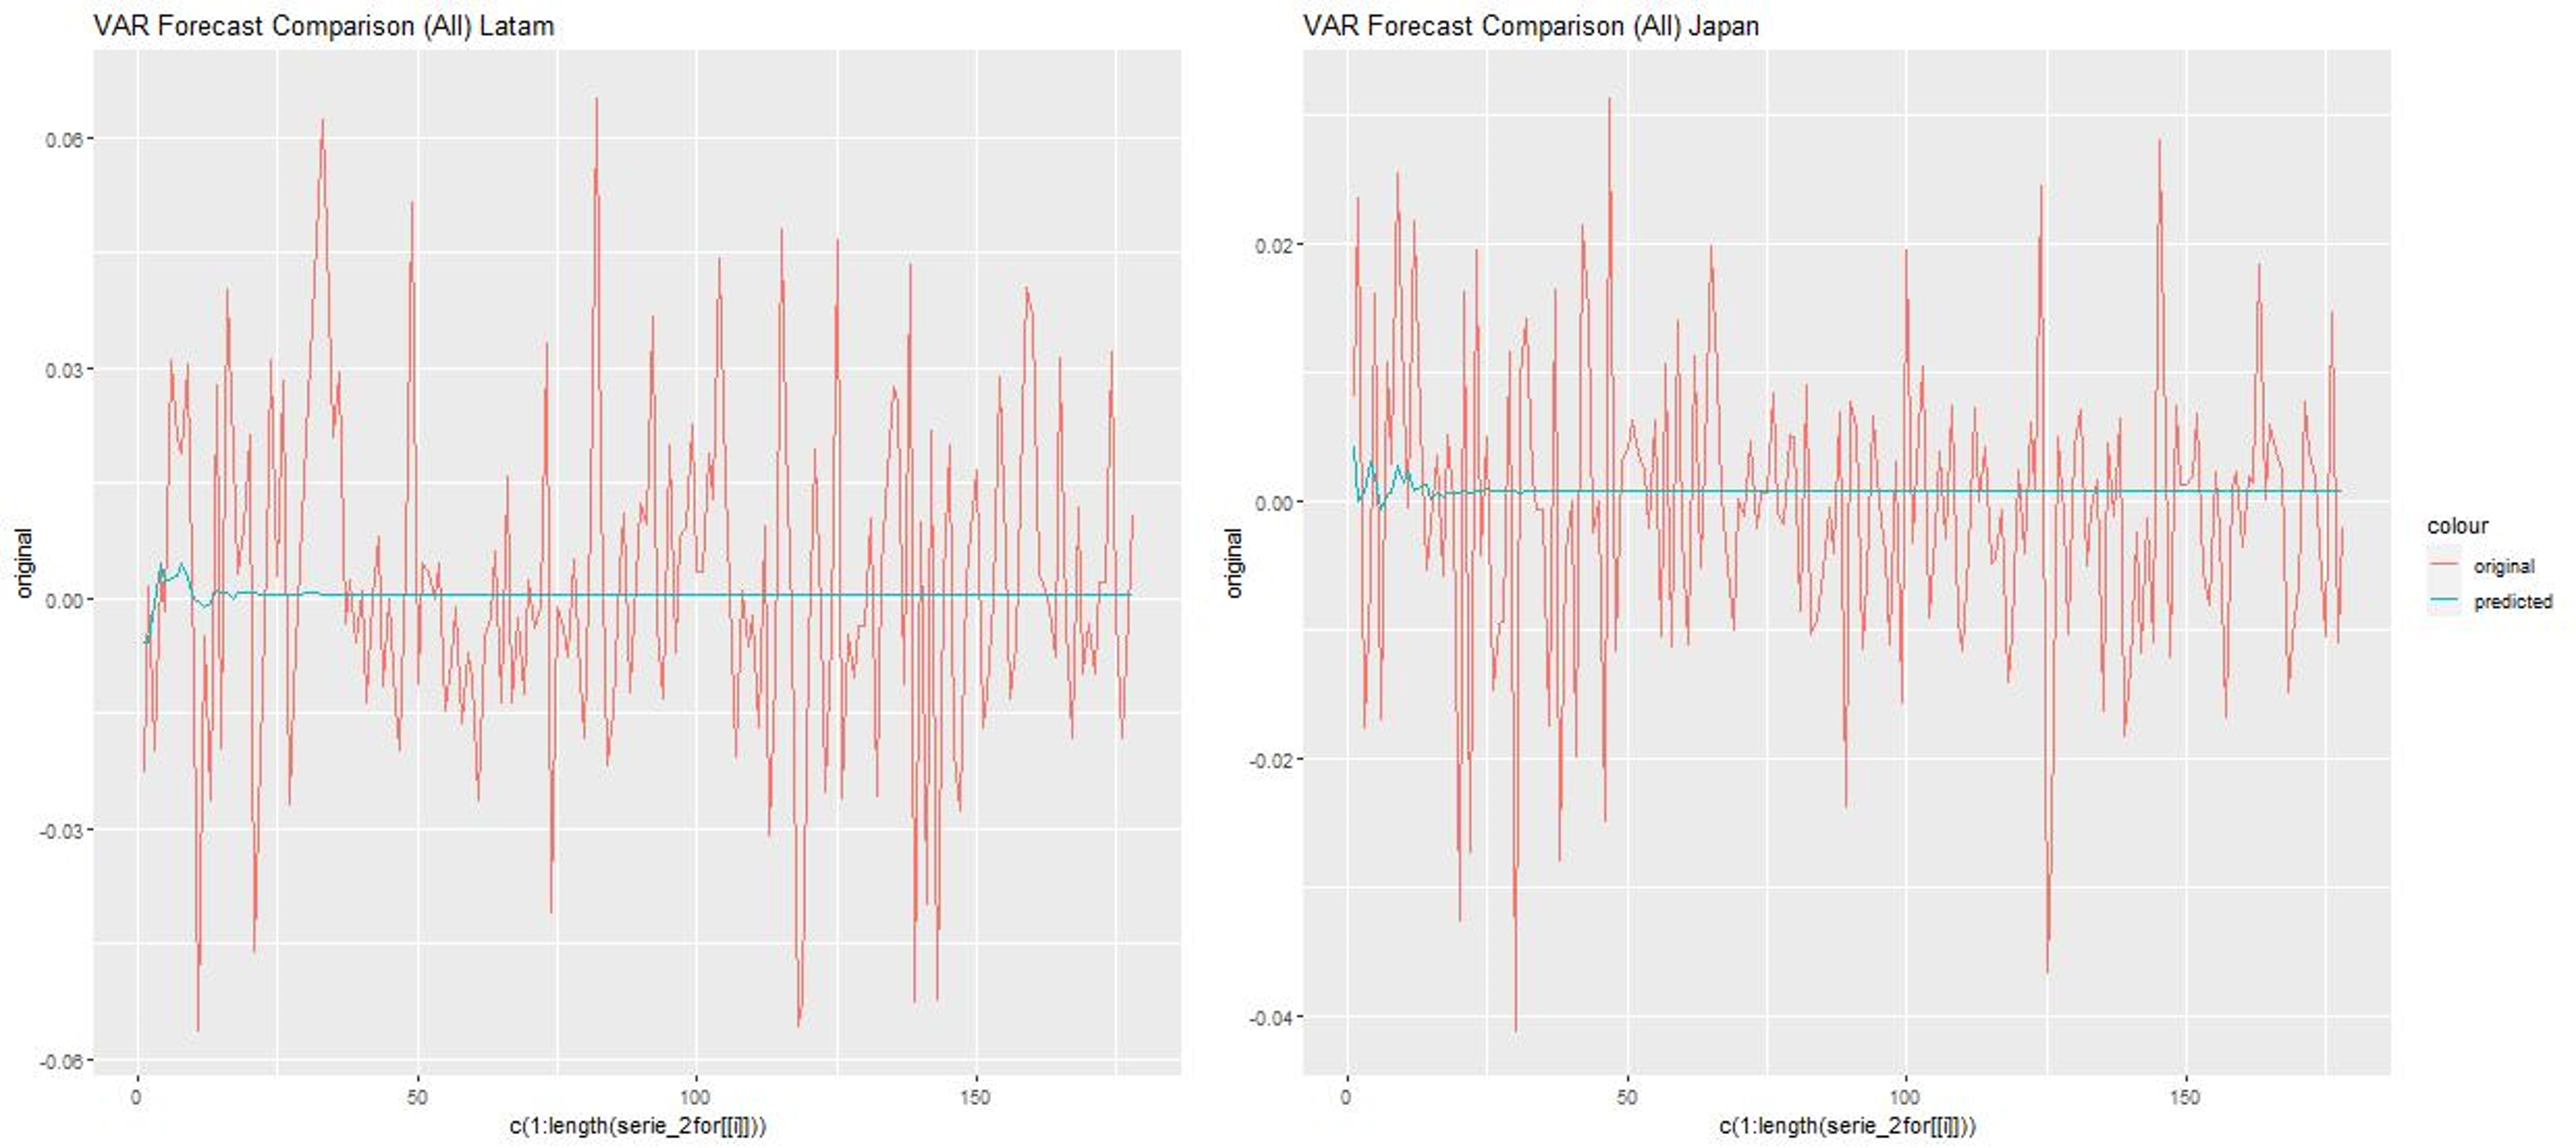
\includegraphics[width=1.0\linewidth]{Imagens/VAR_for_all}
	 	\caption{Previsão do modelo VAR para os 10\% finais das série de Latam e Japan Airlines}
	 	\label{fig:varforall}
	 \end{figure}
	 
	 \begin{figure}[H]
	 	\centering
	 	\includegraphics[width=1.0\linewidth]{Imagens/VAR_for_20}
	 	\caption{Previsão do modelo VAR para os 20 valores finais das série de Latam e Japan Airlines}
	 	\label{fig:varfor20}
	 \end{figure}
	 
	 Por fim, foram calculados os erros RMSE, como definidos na equação \ref{eq:RMSE} e construídas as seguintes tabelas que comparam esses valores para os modelos ARIMA e modelo VAR, tanto para a divisão 90/10 quanto para as 20 entradas finais das series.
	 
	 \begin{table}[H]\label{tab:RMSE_VAR_all}
	 	\centering
	 	
	 	\begin{tabular}{|c|c|c|}
	 		\hline
	 		\multicolumn{3}{|c|}{Erros das previsões para os 10\% finais das séries} \\ \hline
	 		Série                     & RMSE ARIMA             & RMSE VAR            \\ \hline
	 		American                  & 0.02271                & \textcolor{green}{0.01974}             \\
	 		United                    & 0.01319                & 0.02186             \\
	 		Delta                     & 0.01307                & 0.01764             \\
	 		Latam                     & 0.02030                & 0.02167             \\
	 		ChinaSouth                & 0.02005                & \textcolor{green}{0.01925}             \\
	 		ChinaEast                 & 0.02116                & \textcolor{green}{0.01864}             \\
	 		Japan                     & 0.01166                & \textcolor{green}{0.01163}             \\
	 		IAG                       & 0.01997                & 0.02219             \\
	 		Lufthansa                 & 0.01680                & 0.02041             \\
	 		AirFrance-KLM             & 0.01983                & 0.02078             \\ \hline
	 	\end{tabular}
 		\caption{RMSE para divisão 90/10}
	 \end{table}

	 \begin{table}[H]\label{tab:RMSE_VAR_20}
	 	\centering
	 	
	 	\begin{tabular}{|c|c|c|}
	 		\hline
	 		\multicolumn{3}{|c|}{Erros das previsões para os 20 valores finais das séries} \\ \hline
	 		Série              & RMSE ARIMA      & RMSE VAR     \\ \hline
	 		American           & 0.01924                              & 0.02265      \\
	 		United             & 0.01090                              & 0.01780      \\
	 		Delta              & 0.01166                              & 0.01782      \\
	 		Latam              & 0.02063                              & \textcolor{green}{0.01584}      \\
	 		ChinaSouth         & 0.01589                              & 0.02144      \\
	 		ChinaEast          & 0.01773                              & 0.02041      \\
	 		Japan              & 0.00824                              & \textcolor{green}{0.00823}      \\
	 		IAG                & 0.01424                              & 0.01459      \\
	 		Lufthansa          & 0.01061                              & 0.01967      \\
	 		AirFrance-KLM      & 0.01510                              & 0.01931      \\ \hline
	 	\end{tabular}
 		\caption{RMSE para 20 valores finais}
	 \end{table}
 
	 
	\subsubsection{Resultados Interconexões}\label{sec:resultados_VAR_itnerconec}
	
	Dados os resultados obtidos na seção \ref{sec:resultados_VAR_previsao}, podemos partir para os resultados das análises de interconexão discutidas na seção \ref{sec:interconex}. Como comentado, uma das possíveis vantagens de se utilizar um modelo autoregressivo vetorial ao invés de vários modelos AR simples é o fato de podermos buscar interconexões ou relações de dependência entre as séries modeladas.
	
	Ao executar a função \textrm{causality} do pacote \textrm{vars}, que implementa o algoritmo de \textrm{Granger Causality} apresentado na seção \ref{sec:interconex}, são obtidas respostas idênticas para todas as séries. A resposta do teste de causalidade para as séries das companhias Latam e Japan Airlines, por exemplo, estão exibidas abaixo.
	
	\begin{figure}[H]
		\centering
		\includegraphics[width=0.9\linewidth]{Imagens/GrangerCausality}
		\caption{Granger Causality para Latam e Japan Airlines}
		\label{fig:grangercausality}
	\end{figure}
	
	Dado o output dessa função, a interpretação do resultado é clara: nenhuma das séries, embora todas sejam de um mesmo nicho de mercado, apresenta relação de causalidade com as demais.
	
	Partindo para a análise da função de resposta impulsional \textrm{IRF} definida na seção \ref{sec:interconex}, foi utilizada uma função do mesmo pacote com o nome de \textrm{irf} cujo retorno pode ser expressado de maneira visual como a imagem abaixo para a série da Japan Airlines.
	
	\begin{figure}[H]
		\centering
		\includegraphics[width=0.9\linewidth]{Imagens/IRF_Japan}
		\caption{Impulse Response Function para a série da Japan Airlines}
		\label{fig:irfjapan}
	\end{figure}
	
	Para entender este resultado, que também é muito similar entre todas as séries temporais das companhias aéreas, vale lembrar que a resposta impulsional procura medir o comportamento das demais séries quando uma delas sofre um choque abrupto em seus valores. Note, portante, que esse choque na figura \ref{fig:irfjapan} está justamente na companhia Japan. Além disso, note que as demais companhias apresentam algumas oscilações em suas evoluções naturais mas nenhuma com amplitude significativa e todas com curta duração, visto que as oscilações praticamente desaparecem após 15 passos. Desse modo, podemos interpretar este resultado como uma garantia de que, além de não estarem causalmente relacionadas, as séries também possuem grau de independência relevante, uma vez que não respondem aos choques umas das outras.
	
	Por fim, a Decomposição de Vriância do Erro de Previsão foi computada por meio da função \textrm{fevd} também do pacote \textrm{vars} \cite{CRANR}. Novamente, para facilitar a interpretação do resultado, vale lembrar que essa análise busca verificar o grau de importância dos choques de uma série na hora de prever o comportamento de outra. A FEVD constrói uma matriz cujas colunas são as séries e os valores de casa linha explicitam esse grau de importância para a série corrente. A figura \ref{fig:fevdjapan} exibe parte da matriz para o caso da companhia japonesa.
	
	\begin{figure}[H]
		\centering
		\includegraphics[width=1.0\linewidth]{Imagens/FEVD_Japan}
		\caption{Matriz resultante da FEVD para Japan Airlines}
		\label{fig:fevdjapan}
	\end{figure}
	
	Para compreender a matriz da figura \ref{fig:fevdjapan}, note que a segunda coluna, que se refere à companhia Japan, está com todos os valores muito próximos de 1. Isso, assim como explicado na seção \ref{sec:interconex}, é óbvio pois os choque em uma série \textrm{X} devem ser os principais contribuintes para os erros na própria série \textrm{X}. Somado a isso, note que todas as demais entradas para todas as demais colunas são próximas de 0 o que, novamente, faz sentido, haja vista a figura \ref{fig:fevdjapan} que exibe as respostas impulsionais para o caso japonês. Perceba, por fim, que, embora ainda muito pequenos, os valores da terceira coluna, referentes à companhia China Southern são os maiores quando comparados com todas as demais e ao olhar para a resposta impulsional desta companhia quando a Japan sofre um choque também notamos uma amplitude um pouco maior  que das demais logo após o choque. Dito isso, podemos interpretar esse resultado de forma a, mais uma vez, fortalecer a tese de que as 10 séries utilizadas são razoavelmente independentes.
	
	As conclusões mais detalhadas a cerca de todos os resultados apresentados encontram-se na seção \ref{sec:conclusao}.
	
	\subsection{Modelo Hídrido: Wavelets + ARIMA}
	
	Com o intuito de entender a Teoria de Wavelets, é importante trazer uma brevíssima contextualização histórica que explique não só a origem dessa teoria, mas também suas vantagens em relação às teorias anteriores.
	
	A análise de sinais no domínio da frequência tem como grande expoente o desenvolvimento da Análise de Fourier. Inicialmente, J. Fourier constatou que qualquer função periódica de período $2\pi$ pode ser representada como uma soma de senos e cossenos, gerando a \textrm{Série de Fourier} da função \cite{Wave_Graps}:
	\begin{equation*}
		f(x)=a_0+\sum_{k=1}^{\infty}(a_k\cos kx+b_k\sin kx)
	\end{equation*}
	
	Em seguida, esta teoria foi estendida para englobar funções não periódicas com o desenvolvimento da \textrm{Transformada de Fourier}. Uma transformada pode ser entendida como uma "função de funções", isto é, uma relação que leva uma função de um domínio $X$, como o domínio do tempo, por exemplo, para um contradomínio $Y$, como o domínio da frequência, de modo que um sinal qualquer, medido em função do tempo, possa ser analisado sob a perspectiva da frequência. A equação que define a \textrm{Transformada de Fourier}, $F(\xi)$, de um sinal $f(t)$ é
	\begin{equation*}
		F(\xi)=\int_{-\infty}^{\infty}f(t)e^{2\pi i\xi t}dt
	\end{equation*}

	A partir dessa transformada, podemos obter informações referentes à frequência de um sinal que antes apenas fornecia informações temporais. No entanto, não podemos obter ambos os tipos de informação ao mesmo tempo. Ao obter informações acerca da frequência, não sabemos em que momento do tempo ela foi obtida. Esse é um dos pontos em que a Teoria de \textrm{Wavelets} fornecerá vantagens.
	
	A etapa seguinte, e final, da evolução histórica necessária para apresentar o conceito de \textrm{Wavelets} é a \textrm{Short Time Fourier Transform}, ou, como será denominada, \textrm{STFT}. A ideia por detrás dessa transformada é, ao invés de olhar para o sinal como um todo, dividi-lo em segmentos pequenos o suficiente para que sejam estacionários \cite{WaveTutorial}. Para tal, é escolhida uma \textrm{função de janela} de suporte finito e constante que, inicialmente, é colocada no início do sinal e é transladada por toda a sua duração. Essa é uma das ideias utilizadas para o desenvolvimento da teoria de \textrm{Wavelets}. A equação que define a \textrm{STFT} para um sinal $x(t)$ e janela $\omega$ é
	\begin{equation*}
		\textrm{STFT}^{(\omega)}_X(t,f)=\int_{t}[x(t)\omega^{*}(t-t')]e^{2\pi if t}dt
	\end{equation*}

	Uma vez apresentados de forma breve, visto que a Análise de Fourier não é o foco desta pesquisa, podemos, enfim, enumerar alguns desafios que essa teoria não consegue superar e, em seguida, introduzir a teoria de Transformada \textrm{Wavelet} Contínua, ou \textrm{CWT}, que é capaz de suprir essas necessidades.
	
	\begin{enumerate}
		\item Falta de localização temporal: não é possível saber em qual momento do tempo cada frequência existiu
		\item Janela de tamanho fixo: cria uma limitação da análise 
	\end{enumerate}

	Dito isso, a Transformada \textrm{Wavelet} Contínua possui dois parâmetros em sua definição, justamente para superar os desafios enumerados. Um parâmetro é para a captura da informação da frequência, chamado $s$ \textrm{(scale)} que é definido como o inverso da frequência $f$, enquanto o outro, $\tau$ \textrm{(translation)} é responsável por transladar a \textrm{Wavelet}-mãe pelo sinal. A equação que define a \textrm{CWT} é
	\begin{equation}\label{eq:CWT}
		\textrm{CWT}^{\psi}_{x}(\tau,s)=\Psi^{\psi}_x(\tau,s)=\dfrac{1}{\sqrt{s}}\int x(t)\psi^{*}(\dfrac{t-\tau}{s})dt
	\end{equation}

	onde, $s$ e $\tau$ são os parâmetros de escala e translação, $x(t)$ é o sinal original no domínio do tempo, $\psi^*(t)$ é o complexo conjugado da \textrm{Wavelet} mãe. 
	
	Existem diversas funções \textrm{Wavelet} que podem ser utilizadas como \textrm{Wavelet} mãe. É esta função que dará o perfil da curva a ser multiplicada dentro da integral pela função do sinal de entrada. Alguns dos exemplos mais importantes da bibliografia de \textrm{Wavelets} são as família das \textrm{Wavelets} de \textrm{Daubechies}, de \textrm{Coiflet}, de \textrm{Haar} e de \textrm{Symmlet} \cite{Wave_Graps}, exibidas na figura abaixo.
	\begin{figure}[H]
		\centering
		\includegraphics[width=0.7\linewidth]{Imagens/familiasWavelets}
		\caption{Famílias importantes de Wavelets}
		\label{fig:familiaswavelets}
	\end{figure}
	
	Para fins didáticos, vale enumerar os passos utilizados ao computar uma \textrm{CWT} para um sinal qualquer $x(t)$.
	\begin{enumerate}
		\item Posiciona-se a Wavelet mãe $\psi$ no início do sinal $x(t)$, ou seja $\tau=0$. Define-se $s=1$, que é a versão mais comprimida da \textrm{Wavelet}.
		\item A \textrm{Wavelet} na escala 1 e $\tau=0$ é multiplicada pelo sinal e, em seguida, integrada e normalizada.
		\item Translada-se a \textrm{Wavelet} alterando o valor de $\tau$ e repete-se o passo anterior até alcançar ela alcançar o final do sinal.
		\item Incrementa-se o valor de $s$, dilatando o sinal e repetem-se os passos anteriores para todos os valores de $s$ desejados.
		\item A computação para cada valor de $s$ preenche uma linha do plano tempo X frequência (apresentado a seguir)
		\item \textrm{CWT} é obtida quando todos os $s$ são calculados.		
	\end{enumerate}
	
	O resultado final desse procedimento, ou seja, a própria \textrm{CWT}, pode ser visualizado por meio de um plano tempo X frequência como o da figura abaixo.
	\begin{figure}[H]
		\centering
		\includegraphics[width=0.7\linewidth]{Imagens/planoTempoFrequencia}
		\caption{Plano Tempo X Frequência}
		\label{fig:planotempofreq}
	\end{figure}
	
	Uma observação importante que pode ser feita com base na análise deste plano e do conhecimento do \textrm{Princípio de Incerteza de Heisenberg} \cite{WaveTutorial} é a de que, quanto melhor a definição da frequência, pior é a definição do tempo, e vice-versa. Isso quer dizer que, quanto mais para baixo no plano, melhor será a resolução no domínio da frequência e pior no domínio do tempo (note que a altura do retângulo é pequena, quando comparada com a largura). De modo análogo, quanto mais para cima no plano, pior a resolução da frequência e melhor no tempo (note que, agora, a altura dos retângulos é maior que a largura).
	
	A figura abaixo ilustra uma parte do algoritmo descrito acima, onde a curva azul é uma representação da \textrm{Wavelet} mãe e a curva amarela é o sinal original. Note que, da esquerda para a direita, a curva azul é transladada sempre com uma mesma largura ($s$) e, só após passar por todo o sinal, tem sua largura alterada.
	\begin{figure}[H]
		\centering
		\includegraphics[width=0.9\linewidth]{Imagens/passagemOnda}
		\caption{Ilustração do algoritmo de obtenção da CWT}
		\label{fig:passagemonda}
	\end{figure}
	
	Embora a transformada contínua seja de extrema importância para diversas áreas do conhecimento e tenha sido a primeira a ser desenvolvida, é natural que, com o objetivo de implementar rotinas computacionais para a previsão de séries temporais que utilizam a teoria de \textrm{Wavelets}, seja apresentada a \textrm{Transformada Wavelet Discreta}, ou \textrm{DWT}. É esta versão da transformada implementada pelos algoritmos computacionais, visto que o mundo digital é intrinsecamente discreto.
	
	A \textrm{DWT}, diferentemente da sua irmã contínua, não será apresentada como uma equação, mas sim como um algoritmo iterativos de filtros. De certo modo, essa abordagem é mais trivial de ser compreendida do que uma equação matemática pura, uma vez conhecido o conceito de filtro. Dito isso, podemos definir um filtro, de maneira superficial, mas suficiente, como um operador que divide o sinal de entrada em frequências maiores ou menores que uma frequência de corte. Um filtro \textrm{passa-baixas} é aquele que filtra, ou que impede a passagem, das frequências mais altas que a frequência de corte e deixa passar as mais baixas. Um filtro \textrm{passa altas}, por sua vez, faz exatamente o contrário.
	
	Para facilitar o entendimento da implementação do algoritmo da \textrm{DWT}, foi ilustrado um exemplo de uma série $x[n]$ de 512 observações que será a entrada do algoritmo. Na figura, Filtro PB significa passa-baixas, enquanto Filtro PA, passa altas.
	\begin{figure}[H]
		\centering
		\includegraphics[width=0.6\linewidth]{Imagens/DWT}
		\caption{Implementação DWT via filtros}
		\label{fig:dwt}
	\end{figure}
	
	O algoritmo da \textrm{DWT}, para o exemplo da figura \ref{fig:dwt}, funciona da seguinte forma. Uma série de 512 entradas passa por dois filtros: um passa-baixas e outro passa-altas, cuja frequência de corte é 500Hz.A saída de cada filtro vai ter exatamente a metade do tamanho da série de entrada, logo 256 valores. A saída do filtro passa-altas, cujas frequências vão de 500 a 1000 Hz, são os coeficientes da decomposição nesse nível. A saída do passa-baixas, também com 256 valores mas com frequências entre 0 e 500 Hz será a entrada dos filtros do próximo nível de decomposição. Essa iteração deve ser feita até atingir o nível de decomposição desejado ou até a série acabar, visto que, a cada iteração, perde-se metade do tamanho da série.
	
	Ao final do algoritmo, os coeficientes que formam a \textrm{DWT} são as saídas dos filtros passa-altas em cada nível de decomposição e a saída do passa-baixas do último nível.
	
	Note que, a cada iteração, perde-se metade da informação que existia no nível anterior. Isso é um problema significativo, uma vez que esses coeficientes serão tratados como novas séries a serem modeladas via ARIMA. Sendo assim, em níveis mais profundos da decomposição, responsáveis por fornecer informação sobre as baixas frequências, teremos poucas entradas para a modelagem ARIMA, o que pode gerar deficiências na estimativa do modelo e, consequentemente, na qualidade da previsão. A fim de contornar esse problema, existe uma outra transformada \textrm{Wavelet} denominada \textrm{Maximal Overlap Discrete Wavelet Transform}, ou MODWT, que impede a perda de metade da informação a cada nível da decomposição, ou seja, garante que todas as saídas dos filtros possuam uma quantidade constante de entradas \cite{WaveARIMA}. Esta é a transformada utilizada pelo pacote de R que foi utilizado para a obtenção dos resultados a serem apresentados em \ref{sec:resultadosWave}.
	
	Uma vez apresentados os fundamentos teóricos da teoria de \textrm{Wavelets} e conhecida a modelagem ARIMA, estudada na primeira parte desta pesquisa cujo relatório está disponível em \cite{git}, pode ser definido o algoritmo, em alto nível, do modelo híbrido de previsão que combina ARIMA com \textrm{Wavelets}. A imagem a seguir ilustra esse algoritmo, inspirado por \cite{WaveARIMA}.
	\begin{figure}[H]
		\centering
		\includegraphics[width=1.0\linewidth]{Imagens/diagramaModeloHibrido}
		\caption{Diagrama do algoritmo do modelo híbrido ARIMA + Wavelets}
		\label{fig:diagramawaveletsARIMA}
	\end{figure}
	
	A imagem \ref{fig:diagramawaveletsARIMA} mostra que o algoritmo funciona da seguinte maneira. Primeiramente, a série bruta é pré-processada, o que engloba análise de estacionariedade \textrm{(Augmented Dickey-Fuller Test)} \cite{Tsay}, completar valores faltantes e obter o \textrm{log-return} a partir da série original. Uma vez ajustada, a série será decomposta via \textrm{DWT}, ou, melhor dizendo, \textrm{MODWT}. Com o resultado da composição em mãos, cada uma das novas séries obtidas em frequências distintas será modelada via ARIMA e, em seguida, prevista. Por fim, a série original é recuperada via \textrm{DWT} inversa.
	
	O grande objetivo desta pesquisa é verificar se, ao prever as séries decompostas e filtradas em frequências específicas, será obtida uma maior precisão. Ao realizar a previsão via ARIMA para cada uma das decomposições, espera-se que o algoritmo seja capaz de perceber padrões que, na série original, eram imperceptíveis. Por exemplo, uma série pode exibir um perfil oscilatório bem comportado ao longo de anos, ou seja, para frequências menores, e comportamentos semanais, frequências maiores, também muito bem definidos. Embora seja difícil, muitas vezes, para o modelo ARIMA perceber essas diferentes características de uma série, espera-se que, ao decompor os dados originais em séries de frequências distintas, possamos ser capaz de fazê-lo.
	
	A fim de comparar o resultado do algoritmo, foi utilizado o \textrm{RMSE} \textrm{(Root Mean Square Error)} entre os valores previstos e os valores originais separados em um grupo de teste. A definição de \textrm{RMSE}, já apresentada na equação \ref{eq:RMSE}, encontra-se novamente abaixo.
	\begin{equation*}
			\textrm{RMSE} = \sqrt{\dfrac{\sum_{t=1}^{h}(\hat{Y}_t-Y_t)^2}{h}}
	\end{equation*}
	
	\subsection{Resultados Wavelets + ARIMA}\label{sec:resultadosWave}
	
	Com o intuito de implementar o algoritmo de modelagem e previsão do modelo híbrido apresentado na seção anterior, foi utilizada, novamente, a linguagem R pelos mesmos motivos já enumerados. Durante a pesquisa, foi descoberto um pacote dedicado a combinar \textrm{Wavelets} com o modelo ARIMA denominado \textrm{WaveletARIMA} e disponível em \cite{CRANR}. Este pacote fornece apenas duas funções: \textrm{WaveletFitting} e \textrm{WaveletFittingarma}. A segunda função foi aquela utilizada nesta pesquisa e ela implementa o algoritmo da MODWT, utilizando o filtro \textrm{Haar}, para a decomposição \textrm{Wavelet}.
	
	Essa função recebe como parâmetros a série temporal, o nível de decomposição, o horizonte de previsão e o \textrm{lag} máximo para as ordens AR e MA do modelo ARIMA (ver \cite{Tsay} ou relatório anterior em \cite{git}). Como retorno, ela devolve um objeto de classe \textrm{WaveletFittingarma} que é, basicamente, uma lista de listas com todos os coeficientes estimados e valores futuros previstos, além de algumas outras métricas menos importantes para esta pesquisa. Note, portanto, que esta função é responsável todo o processo de decomposição via MODWT, estimativa do modelo ARIMA e previsão, restando apenas o pré processamento e o cálculo do erro da previsão.
	
	Dito isso, o pré-processamento foi feito de forma idêntica ao já apresentado para o modelo VAR e também realizado para o modelo ARIMA da primeira etapa desta pesquisa. De mesmo modo, foram utilizadas exatamente as mesmas séries de todo o restante da pesquisa a fim de obter uma comparação justa dos diferentes modelos. Sendo assim, será feita apenas uma recapitulação breve dos passos do pré-processamento. 
	
	Uma vez importada a série e selecionado apenas o preço ajustado fechado \textrm{AdjClosed} do arquivo \textrm{csv}, em todas as séries foi realizada uma busca e substituição de valores faltantes. As imagens abaixo exibem duas das séries temporais utilizadas.
	
	\begin{figure}[H]
		\centering
		\includegraphics[width=1.0\linewidth]{Imagens/AdjCloseWavelets}
		\caption{Preço fechado ajustado para AirFrance-KLM e American Airlines}
		\label{fig:adjclosewavelets}
	\end{figure}
	
	Em seguida, foi realizado um teste de estacionariedade, o \textrm{Augmented Dickey-Fuller Test}. As imagens acima já levantam a suspeita de que ambas as séries são não-estacionárias, principalmente a série da \textrm{American Airlines}. Para não dependermos apenas do aspecto visual, o resultado do \textrm{ADF Test} de ambas encontra-se abaixo.
	
	\begin{figure}[H]
		\centering
		\includegraphics[width=0.9\linewidth]{Imagens/AdfTestWave}
		\caption{Resultado do \textrm{ADF Test} para AirFrance-KLM e American Airlines}
		\label{fig:adftestwave}
	\end{figure}
	
	O valor que nos interessa á o \textrm{p-value}, que mede a probabilidade da série possuir uma raiz unitária e, consequentemente, ser não estacionária. Percebe-se que a série da \textrm{American}, como suspeitado pela análise visual, é menos estacionária que a da \textrm{AirFrance-KLM}. Uma vez feita essa análise, o próximo passo é obter o \textrm{log-return} dessas séries, uma vez que não estamos interessados no preço da ação em si, mas no seu retorno. É importante, após obter o retorno, executar novamente uma rotina de limpeza, realizada via função \textrm{tsclean}, para procurar e substituir valores faltantes ou inválidos.
	
	As imagens abaixo exibem o retorno-log das mesmas duas séries.
	
	\begin{figure}[H]
		\centering
		\includegraphics[width=1.0\linewidth]{Imagens/LogRetWave}
		\caption{Log-return das séries AirFrance-KLM e American Airlines}
		\label{fig:logretwave}
	\end{figure}
	
	Como essas são, de fato, as séries que nos interessam, foi feito novamente um teste de estacionariedade para verificar se a série precisa ou não ser diferenciada antes de ser decomposta via \textrm{Wavelets} e modelada via ARIMA \cite{Tsay}. Ambas as séries de retorno possuem aparência de estacionárias, o que é confirmado pelo \textrm{ADF-Test} exibido abaixo, onde podemos ver que ambos os \textrm{p-values} são menores de 0.1, concluindo-se que elas são estacionárias e não precisam de diferenciação.
	
	\begin{figure}[H]
		\centering
		\includegraphics[width=0.9\linewidth]{Imagens/AdfTestWave_LOGRET}
		\caption{Resultado do \textrm{ADF Test} para log-retorno de AirFrance-KLM e American Airlines}
		\label{fig:adftestwave_logret}
	\end{figure}
	
	Enfim, as séries foram dividas em grupos de treino e teste que possuem os mesmos objetivos de sempre: o grupo de treino é usado para estimar o modelo e fazer a previsão enquanto o grupo de teste não é apresentado ao modelo e serve para comparar os valores previstos com os originais.
	
	Novamente são feitas duas divisões: a primeira separa 90\% da séries para treino, deixando os 10\% finais para teste enquanto a segunda separa apenas os 20 últimos valores para teste. Essas duas divisões são feitas para comparar a qualidade de previsão para horizontes longos e curtos,respectivamente. O nível máximo de decomposição de cada série foi escolhido a partir do menor número inteiro mais próximo do log do tamanho da série. Além disso, os valores máximos do \textrm{lag} para ambos os valores de AR e MA foram definidos como 15 dado que, ao utilizar o modelo ARIMA, todas as séries apresentaram \textrm{lags} menores que este valor.
	
	Ao fim de cada estimativa, foi construído um gráfico comparando os valores previstos e os valores separados como grupo de teste. As imagens abaixo exibem esses resultados para as duas mesmas companhias aéreas e para ambas as divisões de treino/teste.
	
	\begin{figure}[H]
		\centering
		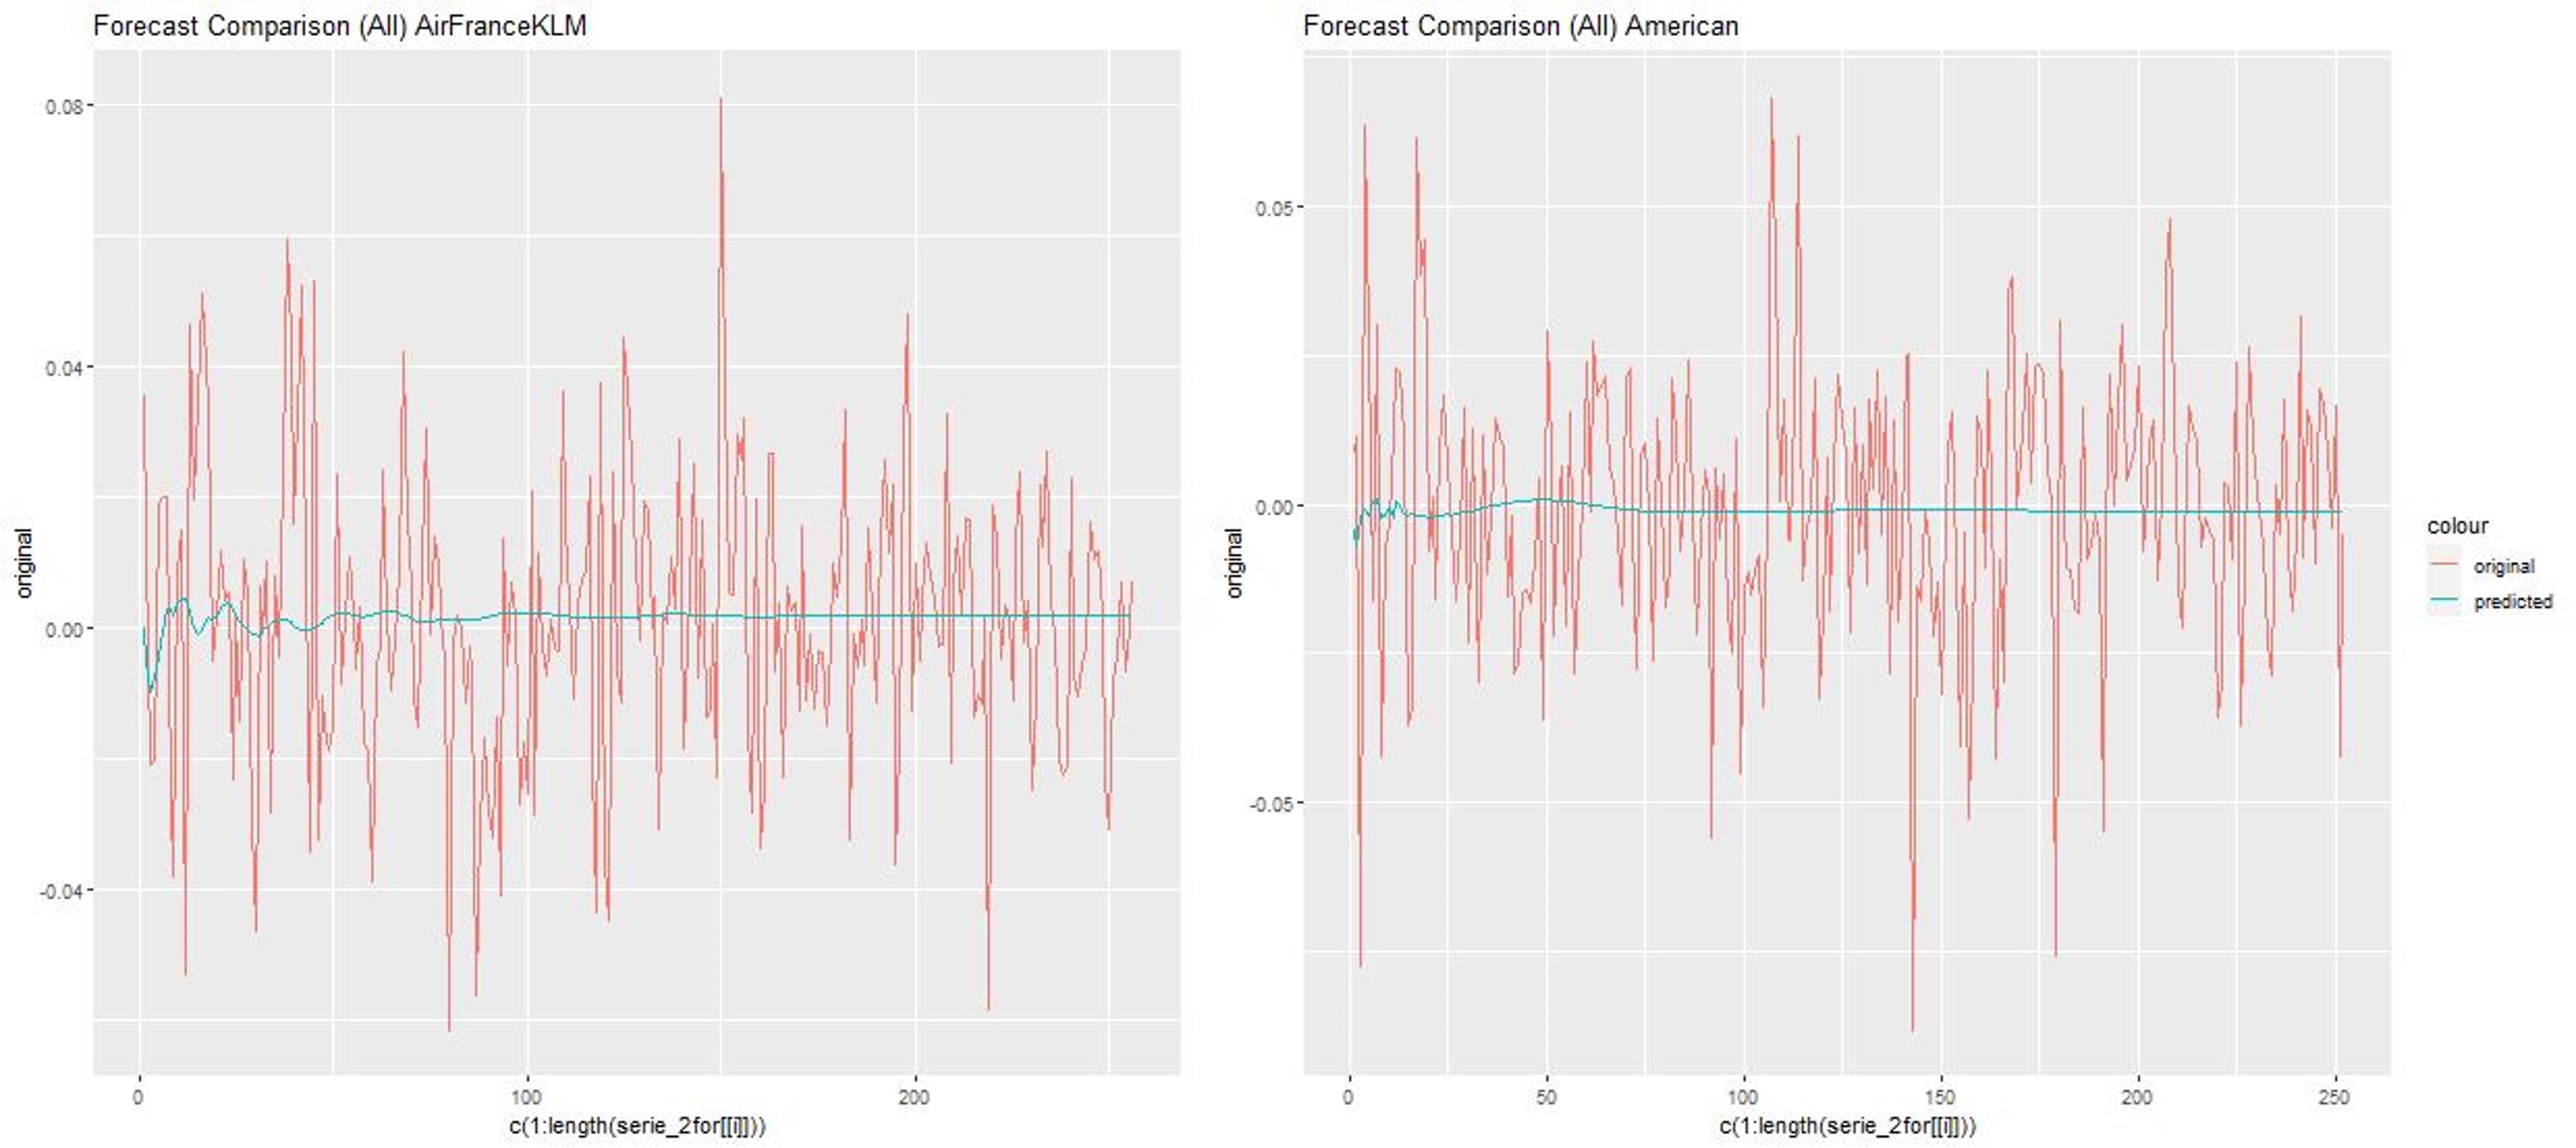
\includegraphics[width=1.0\linewidth]{Imagens/ForWaveAll}
		\caption{Previsão para 10\% finais da AirFrance-KLM e American. Vermelho Original e Azul Previsto}
		\label{fig:forwaveall}
	\end{figure}
	\begin{figure}[H]
		\centering
		\includegraphics[width=1.0\linewidth]{Imagens/ForWave20}
		\caption{Previsão para 20 valores finais da AirFrance-KLM e American. Vermelho Original e Azul Previsto}
		\label{fig:forwave20}
	\end{figure}
	
	Por fim, foi calculado o RMSE entre os valores previstos e os grupos de teste de todas as 10 séries para ambas as divisões implementadas. Esses erros estão exibidos nas tabelas abaixo em comparação com os erros obtidos anteriormente com os modelos ARIMA.
	
	\begin{table}[H]\label{tab:RMSE_Wave_all}
		\centering
		
		\begin{tabular}{|c|c|c|}
			\hline
			\multicolumn{3}{|c|}{Erros das previsões para os 10\% finais das séries} \\ \hline
			Série                 & RMSE ARIMA         & RMSE Wavelets/ARIMA         \\ \hline
			American              & 0.02271            & \textcolor{green}{0.02244}                     \\
			United                & 0.01319            & 0.01445                     \\
			Delta                 & 0.01307            & 0.01342                     \\
			Latam                 & 0.02030            & 0.02411                     \\
			ChinaSouth            & 0.02005            & 0.02307                     \\
			ChinaEast             & 0.02116            & 0.02344                     \\
			Japan                 & 0.01166            & \textcolor{green}{0.01158}                     \\
			IAG                   & 0.01997            & \textcolor{green}{0.01914}                     \\
			Lufthansa             & 0.01680            & \textcolor{green}{0.01653}                     \\
			AirFrance-KLM         & 0.01983            & 0.02191                     \\ \hline
		\end{tabular}
		\caption{RMSE para divisão 90/10}
	\end{table}
	
	\begin{table}[H]\label{tab:RMSE_Wave_20}
		\centering
		
		\begin{tabular}{|c|c|c|}
			\hline
			\multicolumn{3}{|c|}{Erros das previsões para os 20 últimos valores das séries} \\ \hline
			Série                   & RMSE ARIMA           & RMSE Wavelets+ ARIMA           \\ \hline
			American                & 0.01924              & \textcolor{green}{0.01784}                        \\
			United                  & 0.01090              & \textcolor{green}{0.01037}                        \\
			Delta                   & 0.01166              & \textcolor{green}{0.01147}                        \\
			Latam                   & 0.02063              & 0.02220                        \\
			ChinaSouth              & 0.01589              & \textcolor{green}{0.01531}                        \\
			ChinaEast               & 0.01773              & 0.01857                        \\
			Japan                   & 0.00824              & \textcolor{green}{0.00814}                        \\
			IAG                     & 0.01424              & \textcolor{green}{0.01400}                        \\
			Lufthansa               & 0.1061               & 0.01147                        \\
			AirFrance-KLM           & 0.01510              & \textcolor{green}{0.01438}     \\ \hline                  
		\end{tabular}
	\caption{RMSE para 20 últimos valores}
	\end{table}

	As conclusões mais detalhadas a cerca de todos os resultados apresentados encontram-se na seção \ref{sec:conclusao}.
	
	\section{Conclusão}\label{sec:conclusao}
	
	Primeiramente, pode-se notar algo interessante em comum para ambos os modelos VAR e híbrido, que combina \textrm{Wavelets} com o modelo ARIMA. As figuras \ref{fig:varforall}, e \ref{fig:forwaveall} deixam claro que nenhum dos dois modelos é capaz de prever com confiança horizontes muito longos. Em ambos os casos as previsões parecem estabilizar na média após, no máximo, 50 passos à frente. O modelo híbrido, provavelmente devido à decomposição \textrm{Wavelet} que deve encontrar padrões em baixas frequências, ainda exibe alguma oscilação ao longo de todo o horizonte de previsão. No entanto, é uma oscilação extremamente sutil que não pode levar à conclusão de que o modelo é capaz de prever com confiança séries de retornos financeiros por um longo período de tempo.
	
	Dessa forma, partindo para as conclusões sobre o modelo VAR, ao analisar as tabelas 1 e 2 que exibem a comparação dos RMSE para os modelo ARIMA e VAR, percebe-se que houve pouca melhora ao se utilizar o modelo vetorial. Esse resultado, embora a priori possa parecer contra intuitivo, pode ser explicado via resultados apresentados na seção \ref{sec:resultados_VAR_itnerconec}. Ao analisar as possíveis interconexões entre as 10 séries modeladas com VAR, todos os algoritmos deram indícios de que as 10 séries são razoavelmente independentes. Sendo assim, como o modelo não possui informações de relações entre as séries, podemos enxergar o modelo VAR como um simples conjunto de modelos AR que foram computados de forma independente. Esse fato traz uma conclusão plausível para os resultados do RMSE exibidos: para séries pouco relacionadas ou independentes, o modelo VAR não apresenta melhoras na previsão visto que não existe vantagem em analisar em conjunto séries que são independentes. Além disso, percebe-se que em muitos casos o resultado do VAR foi pior do que aquele obtido pelo modelo ARIMA. Um possível motivo para isso é o fato de que, para o modelo vetorial, é definido apenas 1 valor de \textrm{lag} único para todas as séries, enquanto que, ao utilizar o modelo ARIMA, foram definidos valores individuais para cada série, de modo a garantir maior similaridade da estimativa do modelo com o comportamento real da série. Seria interessante, por fim, com o intuito de aumentar a certeza da conclusão em relação à qualidade do modelo VAR para séries independentes, utilizá-lo para modelar e prever séries que são intrinsecamente dependentes ou, no mínimo, assumidamente relacionadas.
	
	Um comentário que deve ser feito é o fato interessante de que, mesmo as 10 séries sendo retornos de ações de empresas de um mesmo nicho - todas são companhias aéreas - a evolução das séries mostra-se independente. Pode-se comentar que o andamento das bolsas em que as ações de cada companhia estão anunciadas sejam distintos uma das outras, mas é, ao meu ver, curioso que nenhum grau de dependência mais significativo do que os resultados apresentados tenha sido obtido. Eventualmente, realizar essa análise para empresas de nichos relacionados e de uma mesma bolsa de valores seria uma análise muito interessante para complementar estes resultados.
	
	Partindo para os resultados do modelo híbrido que combinou a teoria da decomposição de \textrm{Wavelets} com o modelo ARIMA, a principal conclusão, além daquela em relação à previsão de longos horizontes, advém do fato de que, para 20 passos à frente, 7 das 10 séries estudadas apresentaram menor erro em suas previsões. Conclui-se, portanto, que o ferramental poderoso de decomposição em diferentes frequências para a previsão de séries temporais fornece bons resultados quando comparado com modelos clássicos, como os modelos ARIMA e VAR. Como possível continuação ou temas futuros de pesquisa, seria proveitoso testar outros filtros de \textrm{Wavelet}, uma vez que o pacote utilizado apenas implementava para \textrm{Wavelets Haar} e, somado a isso, avaliar esse modelo híbrido para outros tipos de séries temporais, além de comparar seus resultados para séries de retornos financeiros com o modelo GARCH, que é comumente utilizado para a previsão desse tipo de série.
	
	
	
	\bibliographystyle{amsplain, amsalpha}
	\begin{thebibliography}{99} 
		
		\bibitem{Tsay} R. S. Tsay,
		{\bf Analysis of financial time series},
		Third edition. Wiley Series in Probability and Statistics.  John Wiley \& Sons, Inc., Hoboken, NJ.  (2010).
		
		\bibitem{Tsay-Tiao1984} R. S. Tsay and G. C. Tiao,
		{\bf Consistent estimates of autoregressive parameters and extended sample autocorrelation function for stationary and nonstationary ARMA models},
		J. Amer. Statist. Assoc. 79, p.84-96 (1984).
		
		\bibitem{VAR} Zivot, Eric and Wang, Jiahui. Vector autoregressive models for multivariate time series. \textbf{Modeling Financial Time Series with S-Plus} ®, p. 385-429, 2006
		
		\bibitem{WaveARIMA} Bailey, Ken. \textbf{A combined wavelet and ARIMA approach to predicting financial time series.} 2017. Tese de Doutorado. Dublin City University.
		
		\bibitem{WaveTutorial}Polikar, Robi et al. \textbf{The wavelet tutorial.} 1996. UC San Diego, Jacobs School of Engineering.
		
		\bibitem{Wave_Graps}Graps, Amara. \textbf{An introduction to wavelets.} IEEE computational science and engineering, v. 2, n. 2, p. 50-61, 1995.
		
		\bibitem{CRANR} 
		CRAN R Project, \texttt{https://cran.r-project.org/}
		
		\bibitem{git} 
		Github Repository, \texttt{https://github.com/MathNog/UndergraduateResearchProject.git}
		
		
		
	\end{thebibliography}
\end{document}